\subsection{The IoT/Edge Problems}
Resource consumption and orchestration are big problems in the cloud and equally so for the edge. Containers and Kubernetes can be adopted to consume less resources and Kubernetes enables remote orchestration of on-prem nodes. But, because of the heterogeneity of the edge, it faces even more problems. Discussed in this section will be load balancing, protocol conversion and traffic shaping.\\ Not thoroughly discussed in this section will be the issue of ultra low latency. In an updated performance assessments of containers the authors found that containers introduce almost no overhead over a native deployment\cite{felter2015updatedPerformanceContainers}. Hence, gateways running Linux can in most cases use containers without a problem. 

\subsubsection{Load Balancing}
Load balancing in a distributed environment is difficult as the ingress node needs a complete network topology at any given moment in time. This is one of the reasons why Kubernetes refreshes its node status so often. If a external request comes in at the master it needs to know where to forward the traffic. In the previous section \cref{sec:singleVsMultiCluster} \nameref{sec:singleVsMultiCluster} I discussed the advantages and disadvantages of multi-cluster in contrast to single clusters and load balancing is a perfect example why the decision has to be carefully weight. A full Kubernetes cluster on the edge comes with the advantage of having a full control plane on the edge and, thus, being able to do load balacing on the edge, with for example Istio Ingress Gateay. If the master nodes taint were to be removed it could even become part of the operational unit of the cluster.\\
But having a cluster at edge comes with its downside. It needs a lot more management than a single cluster setup. It consumes drastically more resources than having only worker nodes and it needs a stable connection between the cluster nodes to work. But if resource consumption on the master is not an issue Kubernetes coupled with a load balancer provide more features and safeguarding than most other load balancers do. Kubernetes always ensures that pods inside the cluster are healthy and reachable and if a pod goes down, Kubernetes will automatically spawn a new one. The internal load balancer can use this information and always route to an available pod. Other gateways like, Kong API Gateway, can not do this. Also with Istio it becomes possible to do very fine grained traffic routing, somthing I will discuss in the next section \cref{} \nameref{}.\\
Finally, internal load balancing\footnote{Load balancing withing one node.} is possible through normal API gateways and the deployment of multiple pods listening on different ports. For example, one NGINX container could function as load balancer for 5 docker containers in the background. In Kubernetes this could be solved with affinities. As soon as a node runs certain pods, a load balancer could be automotically side loaded.
\subsubsection{Traffic Control and Shaping}
Traffic control and traffic shaping are very interesting edge topics. In Kubernetes each pod can be assigned incoming and outgoing bandwidth rates. But other tools extend this functionality and open up new possibilities. Istio, a service mesh mainly developed for Kubernetes, injects a sidecar proxy to fine tune the traffic of each container. It makes it possible to do rate limiting, control headers, reroute connection, change retries attempts, circuit breaking, mirroring and more while not changing the application code. Additionally, it is also able to encrypt traffic inside the mesh without the application knowing about it and gather all the telemetry data of the cluster. \\
With Kubernetes and tools extending its capabilities it is possible to do both traffic control and traffic shaping on a fine grained level. But, especially Istio, comes at the cost of additional overhead and the operator has to decide if the added functionality are worth the performance hit. Without Istio traffic control and shaping is only possible through the Kubernetes Ingress and thus in multi-cluster solutions.\\
Finally, Kubernetes is only meant to work with the Internet protocol stack and is only meant to operate within the clusters boundaries. So the actual communication with the IoT devices can not be controlled or shaped with Kubernetes. 
\subsubsection{IoT Protocols and Protocol Conversation}
Kubernetes was designed for the Inernet and not for the heterogenity of the edge. This means the IoT gateway must either implement a DHCP server, the IoT device must have a static IP or the communication is facilitate outside Kubernetes realm and then converted by a service to IP. Please note that lower level protocols for establishing a connection between two devices, e.g. Ethernet, Wi-Fi (IEEE-802.11) or Bluetooth, are not discussed at this point. The most common IoT protocols are MQTT, CoAP, AMQP and DDS. In contrast to Internet protocol stack, these technologies do not need to support legacy systems and can thus concentrate on whats important in IoT, very low energy, distribution and memory consumption. I will mainly compare MQTT\cite{MQTT50:online} to CoAP\cite{CoAP—Con75:online} because of the their vast usage and academic literature. \Cref{fig:mqttVsCoap} shows side by side the architecture of MQTT and CoAP. Both are based on machine to machine (m2m) communication and are optimized for the IoT space, but the similarities stop there.
\begin{figure}[h!]
    \centering
    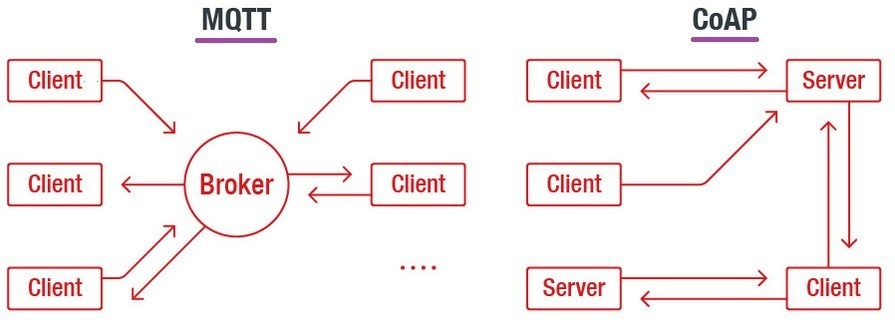
\includegraphics[scale=0.45]{figures/mqtt-vs-coap.jpg}
    \caption{MQTT and CoAP architecture side by side\cite{COAPvsMQTT27:online}.}
    \label{fig:mqttVsCoap}
\end{figure}
MQTT is based on the publish-subscribe massaging pattern which relies on a central entity, called broker, to enable communication between multiple nodes, mainly IoT devices. CoAP on the other side is a classic client server protocol and is based on the Internet stack. Researches compared the two standards and found "MQTT messages experienced lower delays than CoAP for lower packet loss and higher delays than CoAP for higher packet loss"\cite{MQTTvsCoAPAnalysisIEEE}. They also found that the message overhead for small messages is significantly lower at 25\% or less for CoAP compared to MQTT for reliable message transmission. Whereas in MQTT the broker needs additional services to convert the data to Internet compatible standards, CoAP is already able to communicate directly through the Internet. This opens up new possibilities including decentralized communication in subnets.\\
Finally, the data serialization can be even more important than the protocol itself. With the advent of RESTful services JSON soared in popularity. It is human readable but not very space efficient. When researches compared JSON to protobufs they found huge message size differences between the two, shown in \cref{fig:jsonVsProtobufs}.
\begin{figure}[h!]
    \centering
    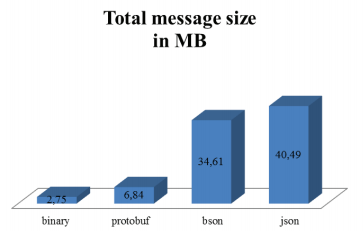
\includegraphics[scale=0.45]{figures/jsonVsProtobufs.png}
    \caption{Memory consumption of different serialization methods\cite{}.}
    \label{fig:jsonVsProtobufs}
\end{figure}
The researches conclude "the Protocol Buffers are a serious candidate for standardized way of communication in field of Internet of Things"\cite{jsonVsProtobufs}.

\comment{
protocol conversation
Traffic shaping
Load balacing
}


